\UseRawInputEncoding
\documentclass[hyperref]{labbook}
\usepackage{hyperref}
\usepackage[utf8]{inputenc}
\usepackage{float}
\usepackage{subcaption}

\usepackage{graphicx}
\begin{document}
\labday{28.12.2020}
\experiment[before]{Measurement of germ content before and after CleanAir use}
\subexperiment{Material}
\begin{itemize}
\item agar plates (Servoplate C3 10413 Nährböden (agars), Sabouraud 2\% Glucose Agar (20-er Pack))
\begin{itemize}
\item pepton: 10g/l
\item D(+) glucose: 20g/l
\item agar: 17g/l
\end{itemize}
\item Kreppband
\end{itemize}
\subexperiment{Baseline}
\begin{itemize}
\item office room - measurements?
\item meeting room table 
\item 6 chairs around table
\item 4 chairs at short wall
\item 1 pot plant
\item window façade at the opposite the wall where CleanAir device was placed
\end{itemize}
\subexperiment{Experimental setup}
\begin{itemize}
\item 4 different distances
\item duplicates
\item incubation time: 47-48min
\end{itemize}
\begin{figure}[H]
\includegraphics[scale=0.28]{cleanair_experiment_schema}
\caption{Schema of office room with the approximate placing of the table, chairs and plant as well as the placing of the CleanAir device. Air flow direction is indicated by the arrows. Agar plates are depicted as brown circles.}
\end{figure}
\begin{table}[H]
\begin{tabular}{|lll|}\hline
Distance from CleanAir  & height from ground & labelling\\\hline
0,4m from suction area & 0m & 28.12., 0,4m, front, before, 1 \\
0,4m from suction area & 0m & 28.12., 0,4m, before, 2 \\
1m from emitting area & 0m & 28.12., 1m, before, back, 1\\
1m from emitting area & 0m & 28.12., 1m, before, back, 2\\
2m & 0,76m & 28.12., 2m, before, 1\\
2m & 0,76m & 28.12., 2m, before, 2\\
4,4m & 0,49m & 28.12., 4,4m, before, 1\\
4,4m & 0m & 28.12., 4,4m, before, 2\\\hline
0,4m from suction area & 0m & 28.12., 0,4m, front, after, 1 \\
0,4m from suction area & 0m & 28.12., 0,4m, after, 2 \\
1m from emitting area & 0m & 28.12., 1m, after, back, 1\\
1m from emitting area & 0m & 28.12., 1m, after, back, 2\\
2m & 0,76m & 28.12., 2m, after, 1\\
2m & 0,76m & 28.12., 2m, after, 2\\
4,4m & 0,49m & 28.12., 4,4m, after, 1\\
4,4m & 0m & 28.12., 4,4m, after, 2\\\hline
\end{tabular}
\caption{plates identifiers}
\end{table}

\subexperiment{Description}

\begin{figure}[H]
\includegraphics[scale=0.05]{_DSC7617}\hfill
\includegraphics[scale=0.05]{_DSC7622}\\
\includegraphics[scale=0.05]{_DSC7623}\hfill
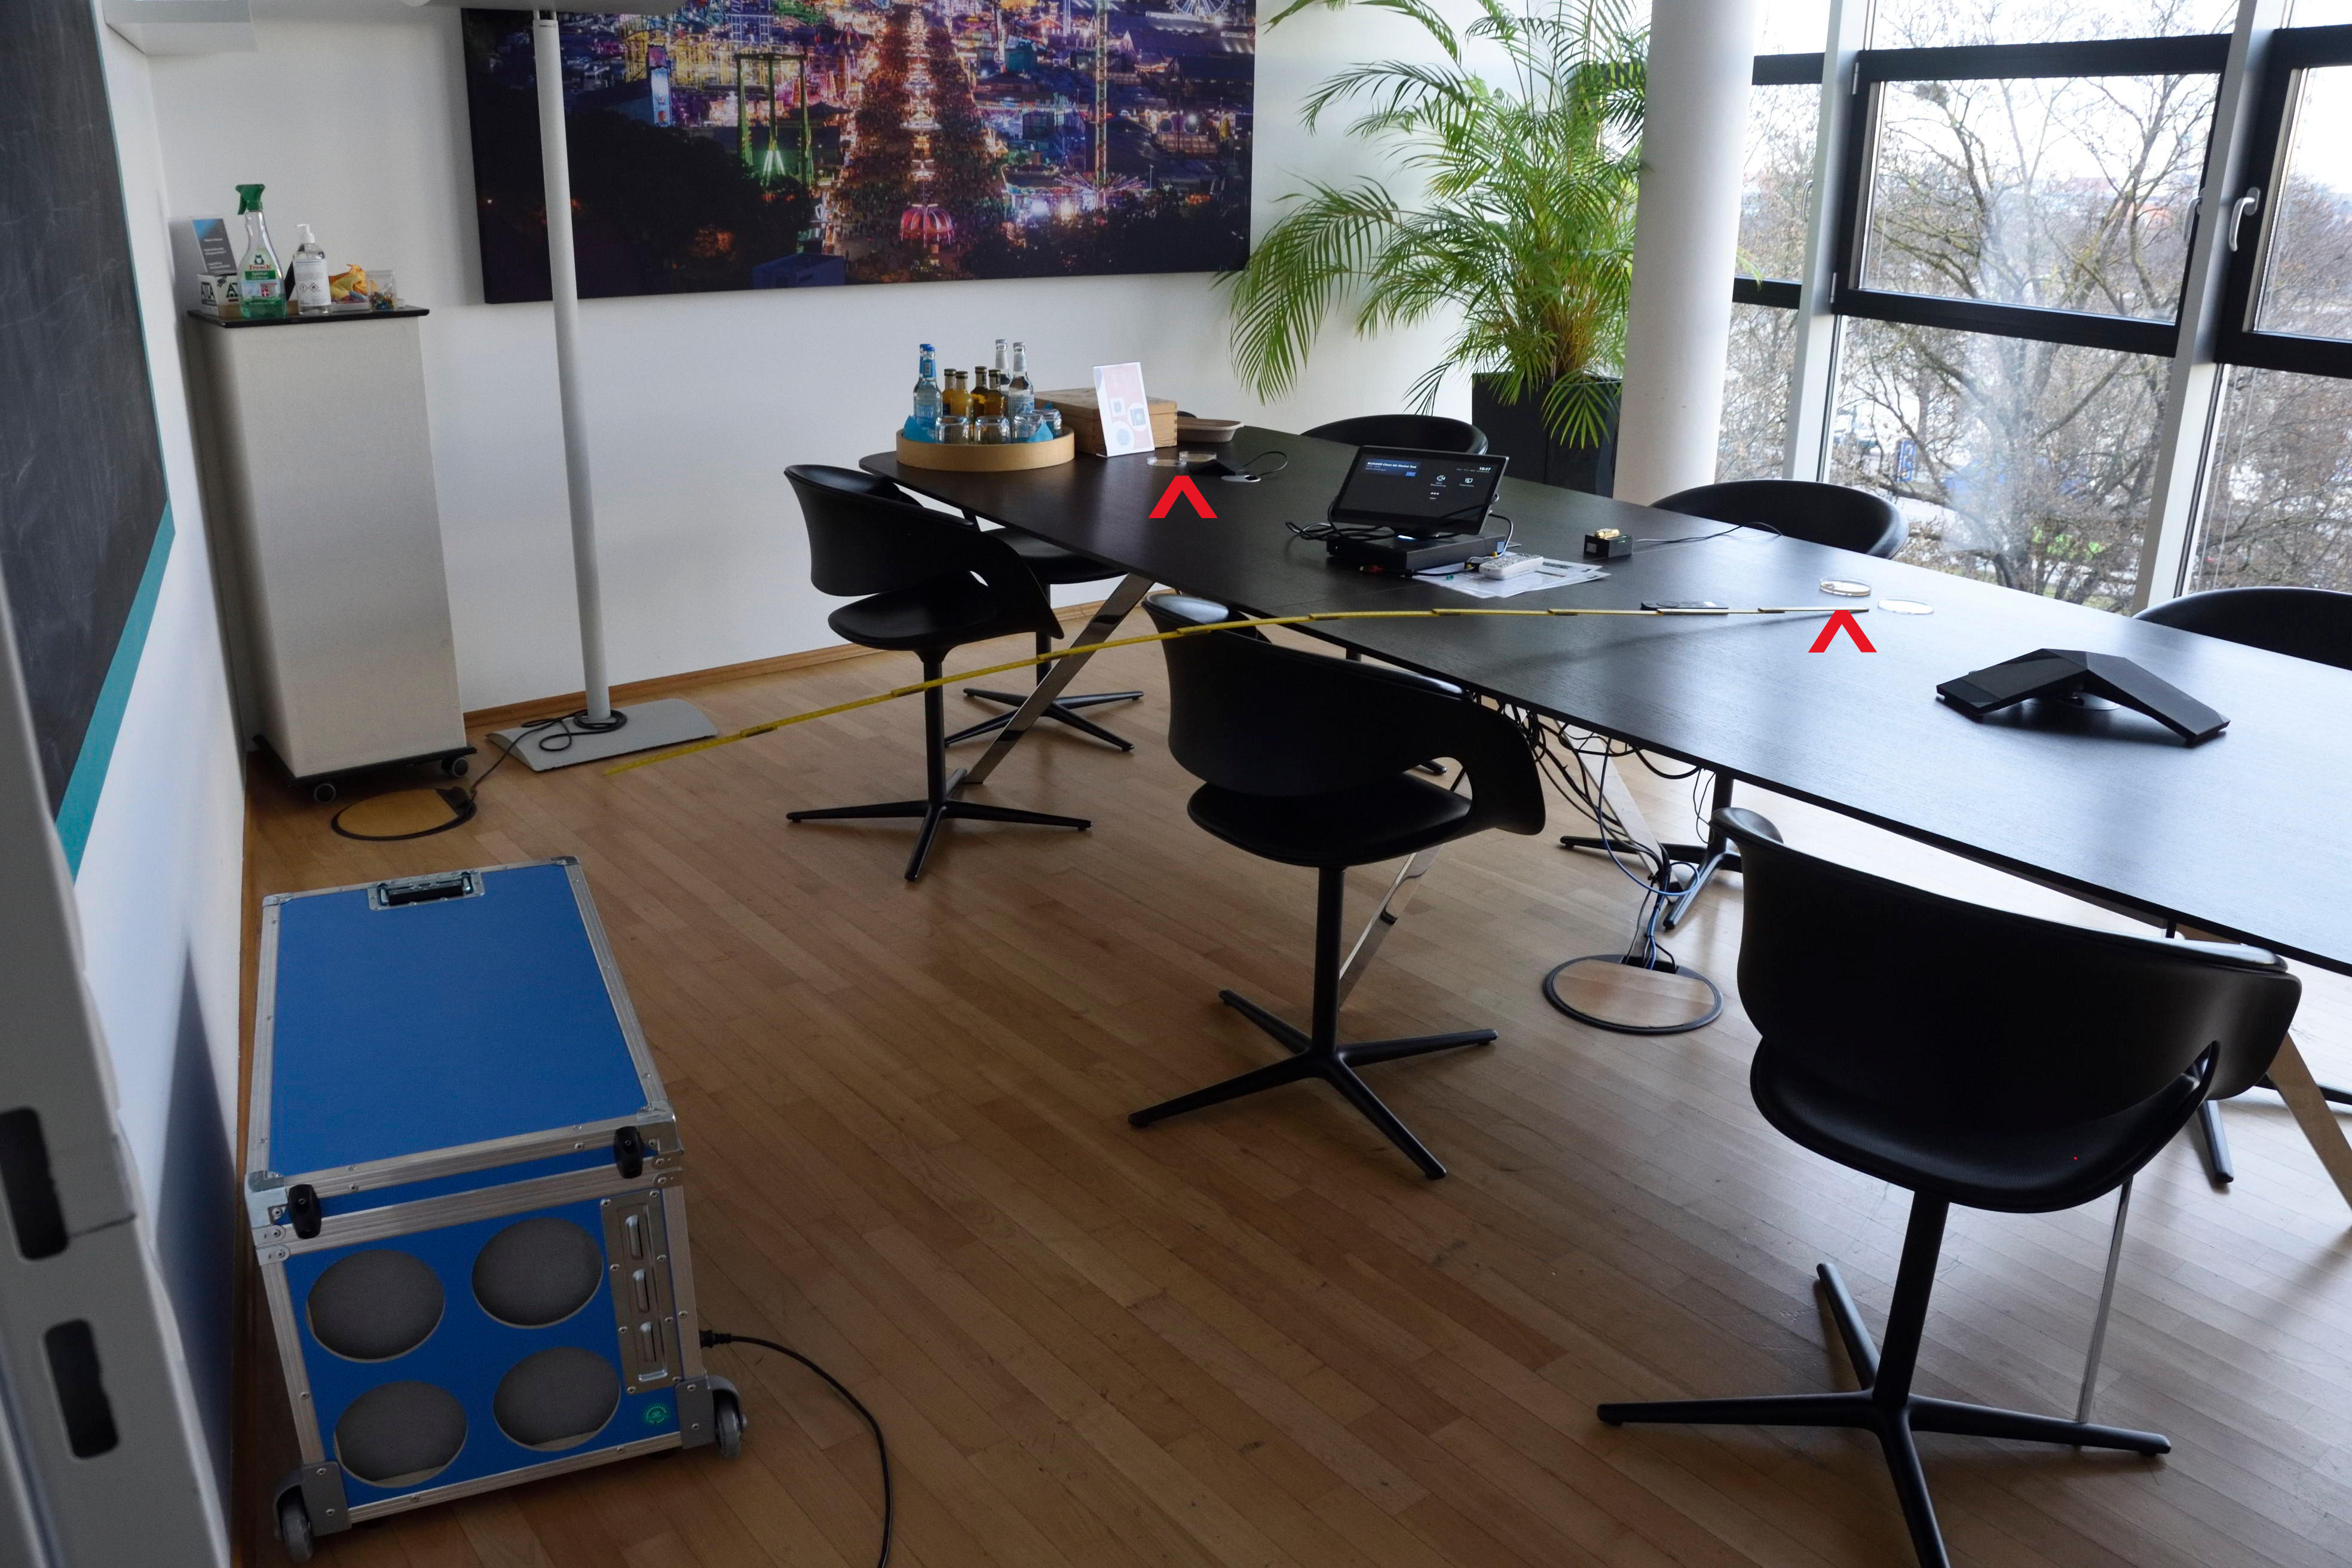
\includegraphics[scale=0.05]{_DSC7624}\\
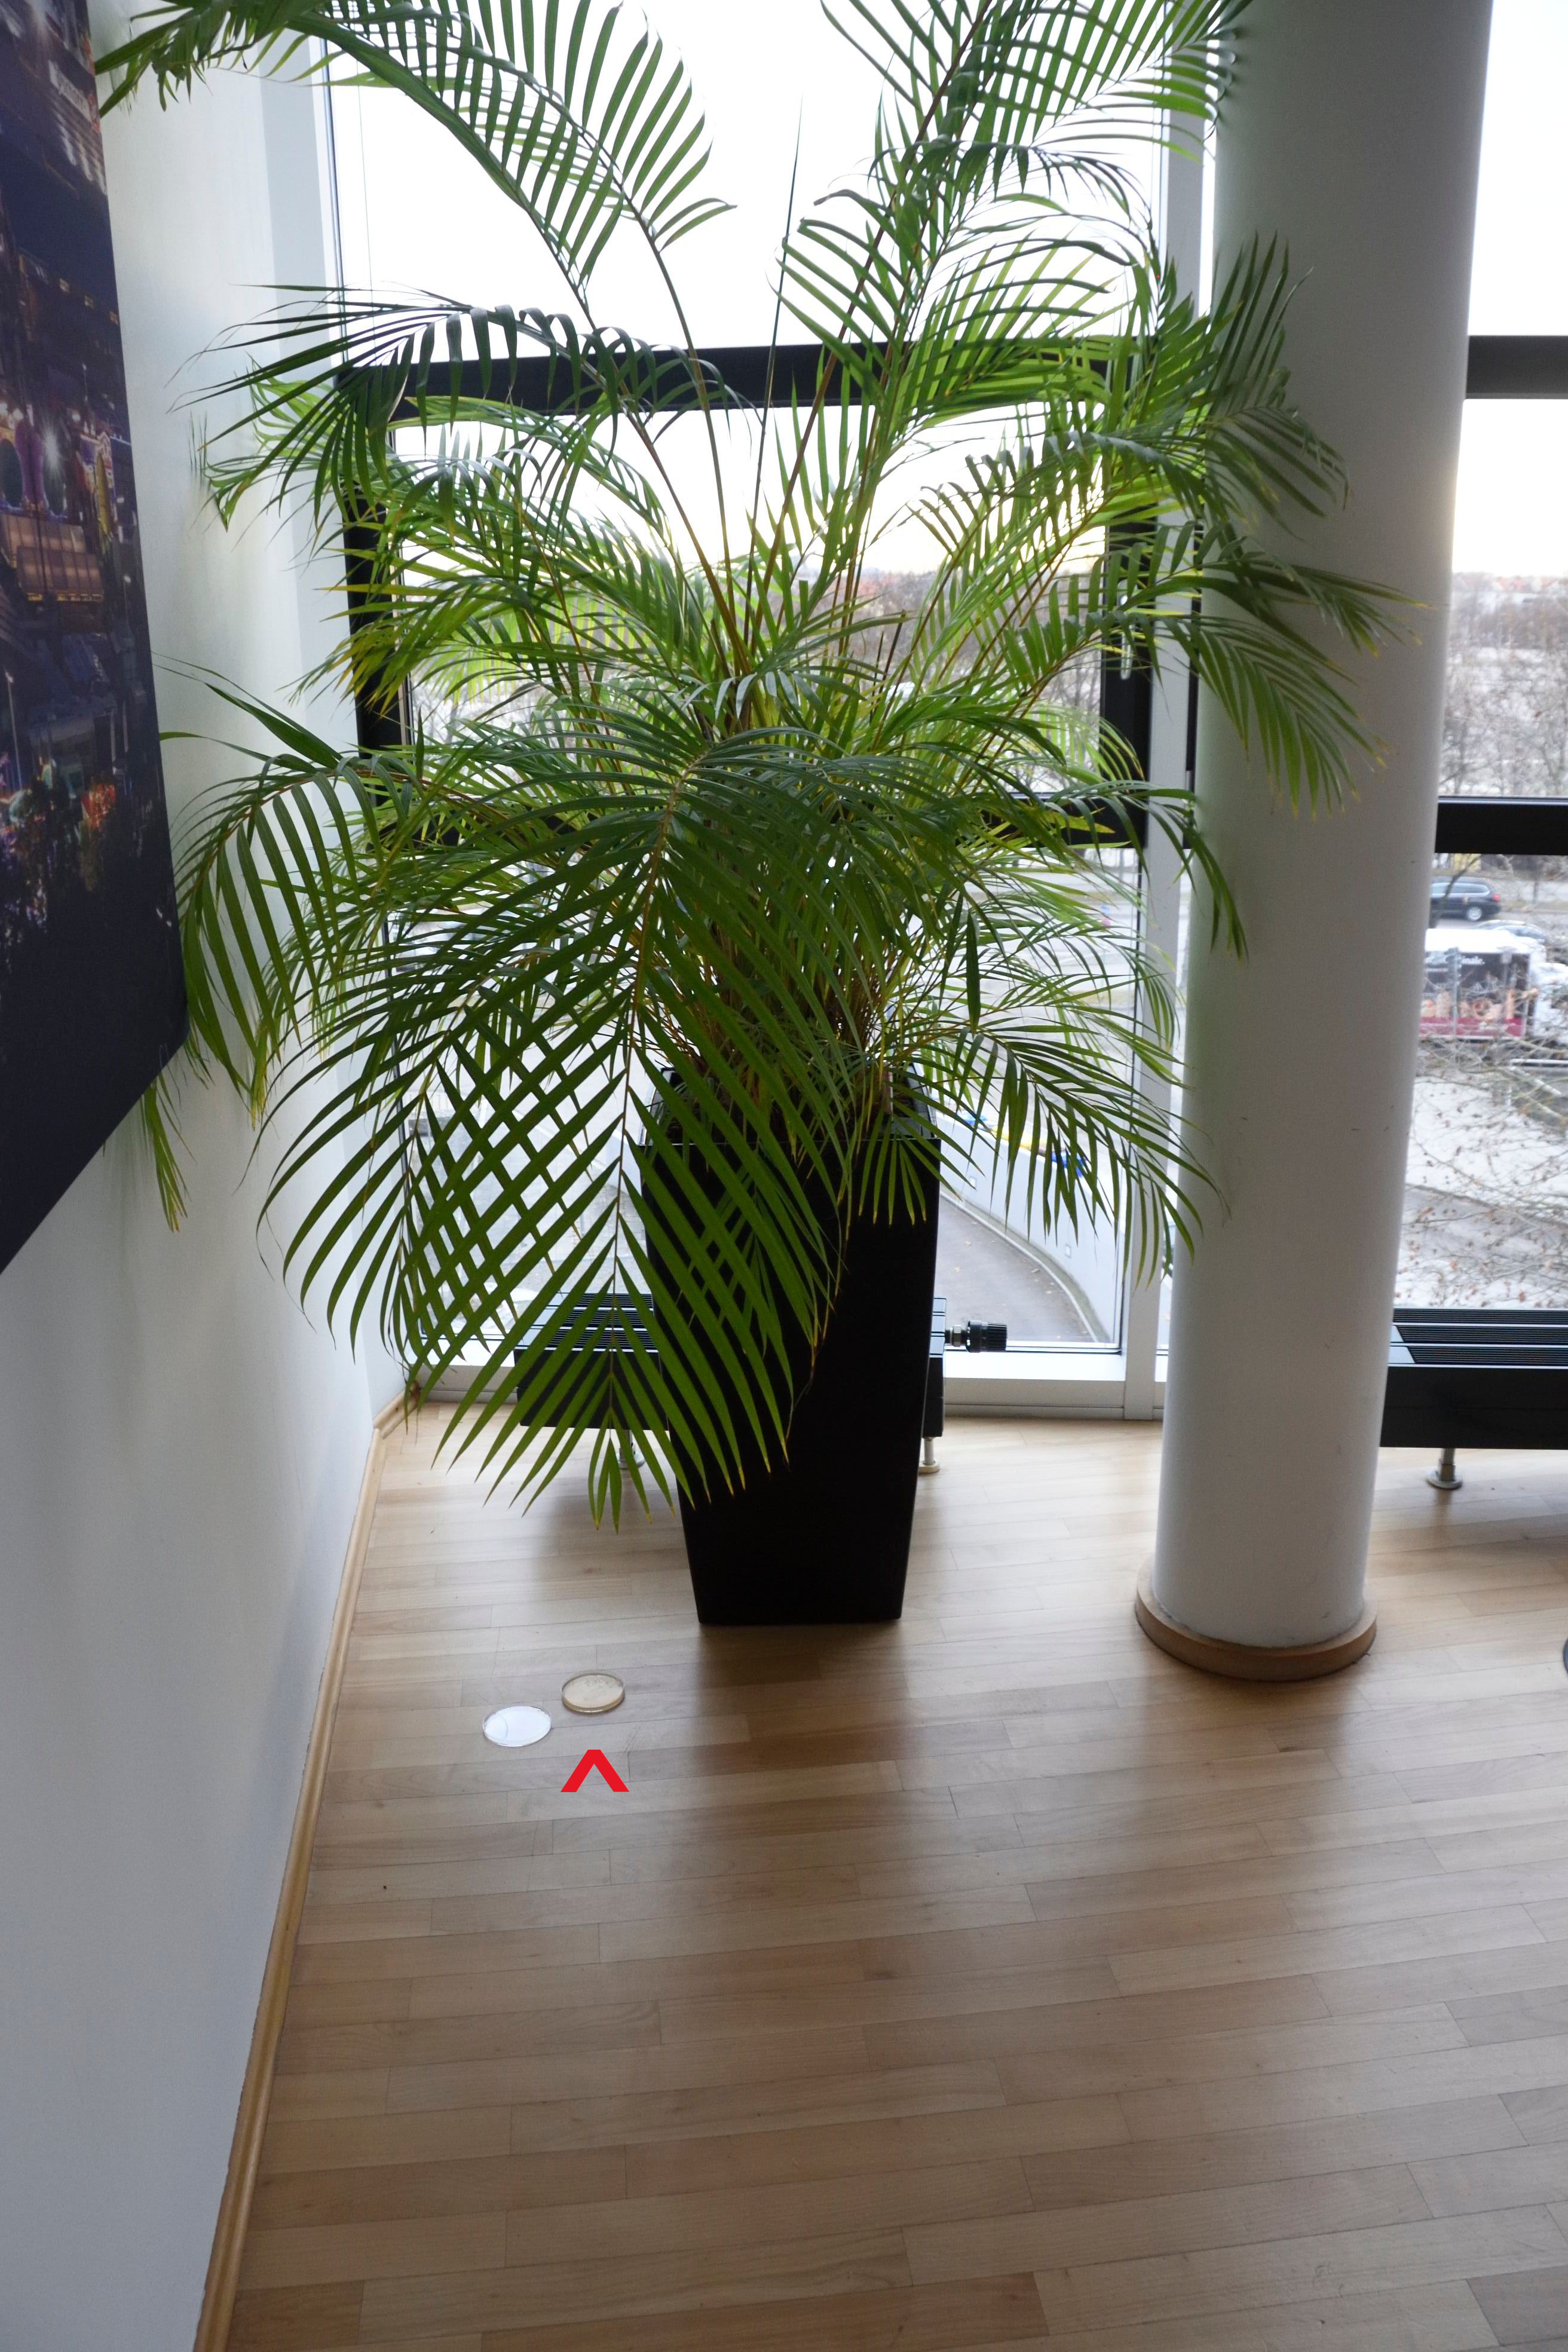
\includegraphics[scale=0.05]{_DSC7621}\\
\caption{photos showing the office and the placement of the CleanAir device and agar plates (red arrows)}
\end{figure}
The office was out of use for one day before starting the experiment. The door was open beforehand. The CleanAir device was placed in the middle of the long wall of the office but was not turned on. Distances were marked using a tape to ensure that before and after measurements are taken from the same location. Plates were placed at the indicated distances from the CleanAir device. Plates were left open for the time of incubation (48min, room temperature). The door was closed during incubation. Starting time of the incubation was 9:56 am, incubation was finished at 10:43 am. The plates were then sealed with tape.\\
The CleanAir device was turned on for 38min at maximum power. The door was closed during air cleaning. (Estimated air turn over rate?)\\
Plates were placed at the indicated distances, the ClearAir device was turned off and plates were left open. The door was opened only shortly and closed immediately before device was turned off and plates were setup. Incubation was at room temperature and started at 11:21 am and ended at 12:09 pm. Plates were sealed with tape.\\
Plates were left at room temperature until colonies are formed. 
\subexperiment{Observations}
\begin{table}[H]
\tiny
\begin{tabular}{|l r | rrrrrrrrr|}\hline
Date      &day&0,4m front I&0,4m front II&1m back I&1m back II&2m I&2m II&4,4m I&4,4m II&Sum\\\hline
28.12.2020&0  &            &             &           &            &    &     &      &       &0  \\
29.12.2020&1  &            &             &           &            &    &     &      &       &0  \\
30.12.2020&2  &            &             &           &            &    &     &      &       &0  \\
31.12.2020&3  &            &             &           &            &    &     &      &       &0  \\
1.1.2021  &4  &            &2            &1          &            &    &1    &      &1      &5  \\
2.1.2021  &5  &1           &2            &1          &            &    &2    &1     &1      &8  \\
3.1.2021  &6  &1           &2            &2          &2           &    &2    &1     &1      &11 \\
4.1.2021  &7  &1           &2            &2          &3           &1   &2    &1     &1      &13 \\
5.1.2021  &8  &5           &2            &2          &3           &2   &3    &1     &1      &19 \\
6.1.2021  &9  &13          &2            &6          &3           &2   &3    &1     &1      &31 \\
7.1.2021  &10 &14          &2            &10         &3           &3   &4    &1     &1      &38 \\
8.1.2021  &11 &14          &2            &10         &3           &3   &4    &1     &1      &38 \\
6.1.2021  &9  &13          &2            &6          &3           &2   &3    &1     &1      &31 \\
7.1.2021  &10 &14          &2            &10         &3           &3   &4    &1     &1      &38 \\
8.1.2021  &11 &14          &2            &10         &3           &3   &4    &1     &1      &38 \\
9.1.2021  &12 &14          &2            &12         &3           &3   &4    &1     &1      &40 \\
10.1.2021 &13 &15          &2            &13         &3           &3   &4    &1     &1      &41 \\
11.1.2021 &14 &15          &2            &13         &3           &3   &4    &1     &1      &41 \\
12.1.2021 &15 &15          &2            &13         &3           &11  &4    &1     &1      &49 \\\hline
\end{tabular}
\caption{Daily counting of CFUs for agar plates placed before CleanAir device was run}
\end{table}
\begin{table}[H]
\tiny
\begin{tabular}{|l r | rrrrrrrrr|}\hline
Date      &day&0,4m front I&0,4m front II&1m back I&1m back II&2m I&2m II&4,4m I&4,4m II&Sum\\\hline
28.12.2020&0  &            &             &           &            &    &     &      &       &0  \\
29.12.2020&1  &            &             &           &            &    &     &      &       &0  \\
30.12.2020&2  &            &             &           &            &    &     &      &       &0  \\
31.12.2020&3  &            &             &           &            &    &     &      &       &0  \\
1.1.2021  &4  &            &1            &           &            &    &     &      &       &1  \\
2.1.2021  &5  &            &1            &1          &            &    &     &      &       &2  \\
3.1.2021  &6  &1           &1            &1          &            &    &     &      &       &3  \\
4.1.2021  &7  &2           &1            &1          &            &    &     &1     &       &5  \\
5.1.2021  &8  &3           &2            &1          &            &    &     &1     &       &7  \\
6.1.2021  &9  &3           &3            &1          &            &    &     &1     &       &8  \\
7.1.2021  &10 &4           &3            &2          &            &    &     &4     &       &13 \\
8.1.2021  &11 &4           &3            &2          &2           &    &1    &4     &       &15 \\
6.1.2021  &9  &3           &3            &1          &            &    &     &1     &       &8  \\
7.1.2021  &10 &4           &3            &2          &            &    &     &4     &       &13 \\
8.1.2021  &11 &4           &3            &2          &2           &    &1    &4     &       &15 \\
9.1.2021  &12 &4           &3            &2          &2           &    &1    &5     &       &16 \\
10.1.2021 &13 &4           &3            &2          &4           &    &1    &6     &       &19 \\
11.1.2021 &14 &4           &3            &2          &5           &    &1    &6     &       &19 \\
12.1.2021 &15 &4           &3            &2          &5           &    &1    &8     &       &22 \\\hline
\end{tabular}
\caption{Daily counting of CFUs for agar plates placed after CleanAir device was run}
\end{table}
\begin{itemize}
\item first CFUs were found at day 4 for both experimental setups
\item funghi are nearly only found in the setup before clean air device was run
\item CFUs in the post clean air experiment are smaller and slower growing
\item possible reasons:
\begin{itemize}
\item these are more resilient bacteria, perhaps spore forming bacteria
\item bacteria are weakened
\end{itemize}
\item CFUs in post clean air experiment are found predominantly in plates that were located near the doors
\begin{itemize}
\item could be brought in through door when device was turned off and plates were placed
\item bacteria were "on the way" to get to the device when air flow was stopped
\end{itemize}
\end{itemize}
possible species in agar plates:
\begin{itemize}
\item \textit{Staphylococcus aureus} root-like structure, yellow, also on human skin, thus can be also air-borne
\item \textit{Micrococcus luteus} yellow, round colonies, typical air-borne bacteria, also on human skin
\item \textit{Penicilium spec.} funghi colonies, very common
\end{itemize}

Except for the plates placed the farthest away from the CleanAir device, all comparable distances show higher CFU numbers in the pre condition. There is a gradient of CFUs from door to window in the pre condition. Except for the plates at 4.4m there is a reduction of CFUs of about one third to one half. The overall number of CFUs after the clean air run is about half as much as that before the device was run. However numbers are small for stable results.
\newpage

\begin{figure}[H]
\begin{subfigure}{\textwidth}
\includegraphics[scale=0.5]{CFU_per_day}
\caption{Median number of CFUs per distance per day}
\end{subfigure}
\begin{subfigure}{\textwidth}
\includegraphics[scale=0.5]{mean_CFU_per_day}
\caption{Mean number of CFUs per condition per day}
\end{subfigure}
\caption{number of colonies over course of observation}
\end{figure}

possible shortcomings:
\begin{itemize}
\item agar plates are for dermatophytic microbes, so some microbes might not grow on this medium that might be able to colonize other human organs
\item CFUs cannot be unambigously classified
\item only qualitative outcome (quantitative results could be obtained through air samplers)
\item no direct measurement of virus possible
\end{itemize}
advantages:
\begin{itemize}
\item can be done easily in any room and setup
\end{itemize}
\end{document}